\documentclass[12pt]{article}

% Margins
\usepackage[letterpaper, top=1in, bottom=1in, left=.5in, right=.5in]{geometry}

% For prettier tables
\usepackage{array}

\usepackage{graphicx}

\usepackage{caption}

\usepackage{float}

% For code
\usepackage{courier}
\usepackage{listings}
\lstset{ mathescape }
\lstset{basicstyle=\ttfamily\footnotesize,breaklines=true}

\usepackage{hyperref}

% Change Font
\usepackage[sfdefault]{roboto}  %% Option 'sfdefault' only if the base font of the document is to be sans serif
\usepackage[T1]{fontenc}

% For double spacing
\usepackage{setspace}

\usepackage[english]{babel}
\usepackage[utf8]{inputenc}
\usepackage{fancyhdr}

\pagenumbering{arabic}

\pagestyle{fancy}
\rhead{Jimmy Hickey}

\lhead{Draft II}


%opening
\title{
Machine Learning Algorithms to Correct Images to Help the Color Blind: Draft II
}
\author{Jimmy Hickey}



\begin{document}
\maketitle
\doublespacing

\begin{abstract}
Many people suffer from color deficient vision; though they learn to cope, they still have many issues distinguishing between colors. In this research, machine learning algorithms are combinted to help to eliminate some of the problems faced by these individuals. As a prototype, specialized data with intentional color blind issues is generated, transformed, and used to train the system. The colors in these images are then segmented using k-means clustering. The image is then analyzed and corrected if neighboring clusters are found to be conflicting. After correcting, the image is more color blind friendly. Omitted from the prototype is a supervised neural network that will be trained to predict these clusters, allowing this process to be applied on any image.

\end{abstract}

\section{Introduction}

Color blindness is a deficiency in a person's color vision. A color blind person will often confuse different colors that a person with normal vision would not have trouble distinguishing. The most common type of color blindness is red-green, followed by blue-yellow, and the rare full lack of color vision. Red-green color blindness affects "as many as 8 percent of men and 0.5 percent of women with Northern European ancestry." \cite{NEI} The effects of color blindness range from minor disruptions such as choosing a mismatched outfit to more major difficulties such as discerning between the colors of traffic lights.
There is no cure for color blindness, however there exist some methods to alleviate symptoms. 

One popular solution to color blindness is specialized glasses. \cite{MITGlasses} The company enchroma sells a variety of these glasses. Color vision starts in the cones of the eye, of which people have three varieties: green, red, and blue. These detect and distinguish between different wavelengths of light; however, in the eye of a color blind person, this discrimination is not always made properly. The enchroma glasses filter out the overlapping wavelengths, making distinctions (particularly between red and green) clearer. These glasses range from \$349 to \$429 without prescriptions and are not ``intended to help pass color blindness tests for occupational purposes."\cite{enchroma} Additionally, they (enchroma brand) are not useful to people with blue-yellow color blindness. A more permanent solution is currently being tested as well.

There is experimental gene therapy that has produced promising results in animals.\cite{MITMonkey} In one study squirrel monkeys, which are naturally red-green color blind, were made able to perceive differences in the two colors after treatment. These animals were monitored and ``retained their new tricolor sensory capacity for more than two years." \cite{MITMonkey}. Additionally, there have been no detected harmful side effects from the treatment; four more animals have been successfully treated since. These auspicious trials suggest that there may be a permanent fix to color blindness in the near future; however, gene therapy is often prohibitively expensive, costings hundreds of thousands of dollars per patient. A short-term, cheap solution to some of the issues faced by the color blind is needed. 

The burgeoning field of computer vision lends itself well to this problem. Much work has been done in the area of feature recognition. Projects like Google's Deep Dream and work in robotic vision are some of the wide applications of computer vision. Computers' abilities to analyze images is greatly enhancing. These methods can be used as the small, cheap fix to some color blind issues. A first step would be to examine images.

Instead of recognizing complex features, a machine needs only to examine the colors in an image. With appropriate knowledge of the problem domain, it should be able to diagnose whether there is areas of the image that may cause issues for the color blind. For example, given a set of color blind tests, it would be able to tell which slides a color blind person would have trouble with. This process can then be incrementally furthered. The system can

\singlespacing
\begin{enumerate}
	\item mark all problem areas.
	\item fix the problem areas without losing too much of the context of the image.
	\item perform the preceding actions on a video.
	\item perform the preceding actions on a live video feed.
\end{enumerate}
\doublespacing

For the scope of this project, the first and second object will be addressed. Unlike the glasses, the machine is not dealing with the light itself, but how it is displayed. Thus, this could be easily expanded to support all of the common types of color blindness. 

The overall goal of this research is to create a prototype to prove that a system can be trained to identify and resolve areas of potential color blind confusion in images.


\section{Methods}

\subsection{Data Creation}
\subsubsection{Image Creation}
Initially, it was planned to use standard Ishihara Color Test plates, such as those used by eye doctors, as the data for this experiment. See figure \ref{fig:ishi} for an example. However, this afforded little control of the data. The learning process would rely on only the Ishihara samples publicly available online. 

\begin{figure}[H]
	\centering
	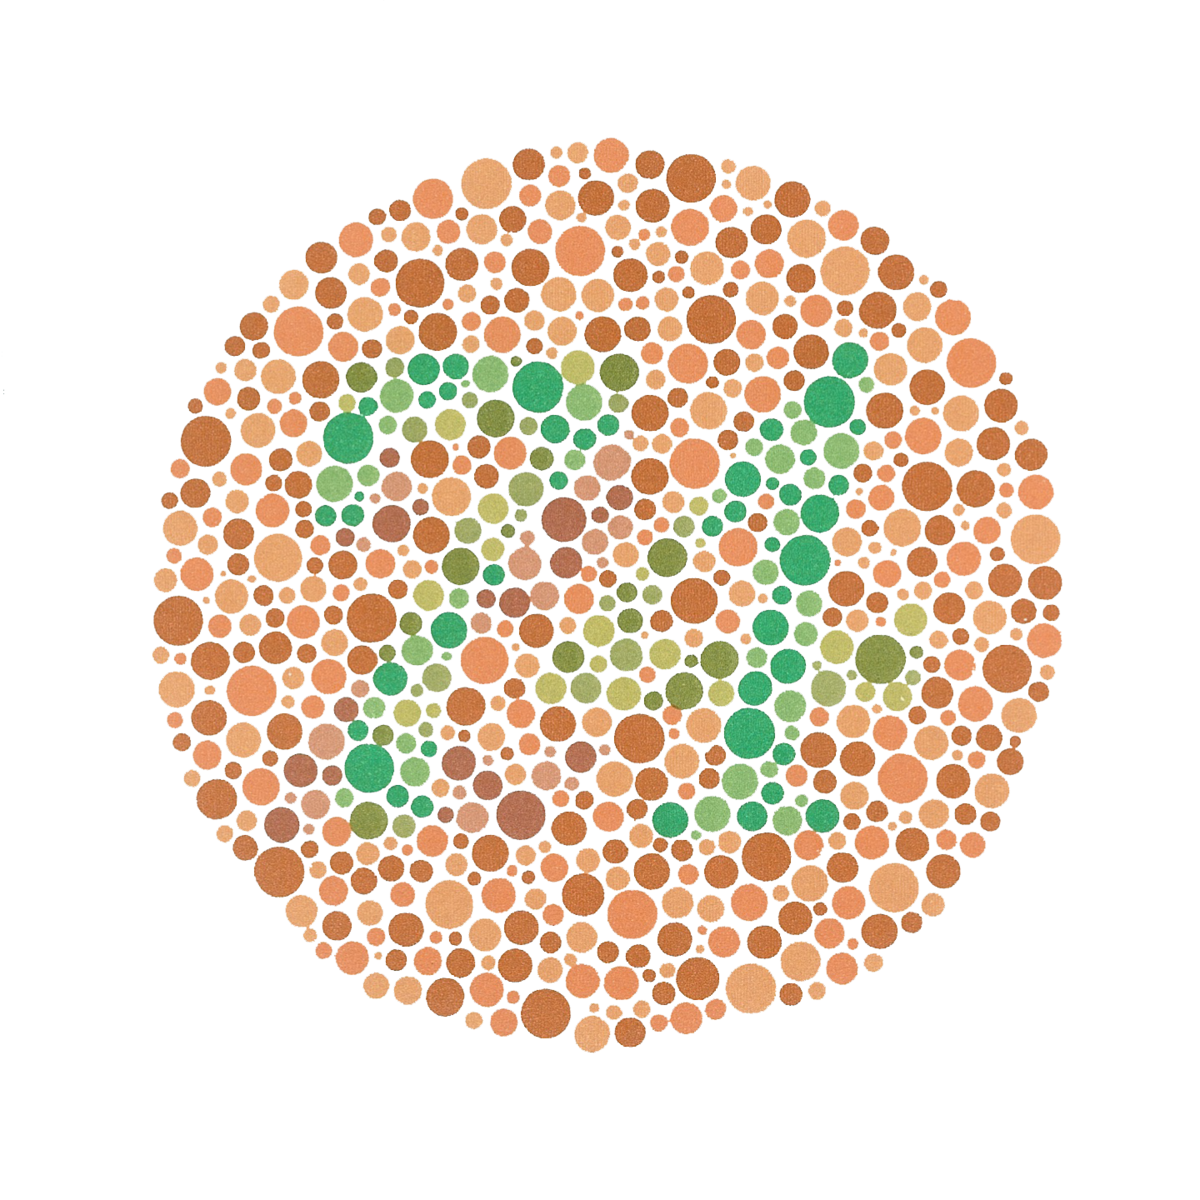
\includegraphics[width=0.25\textwidth]{img/Ishihara}
	\caption{A red-green Ishihara color blind plate.}
	\captionsetup{font={footnotesize,bf,it}}
	\caption*{\href{https://en.wikipedia.org/wiki/Ishihara\_test}{https://en.wikipedia.org/wiki/Ishihara\_test}}
	\label{fig:ishi}
\end{figure}


Instead of this, new data was generated for the sake of this experiment. This allows for a wider range of data to be created and manipulated to help the system learn more color combinations. The data created using Adobe Illustrator. A background was chosen and then a foreground image was drawn. The colors of the background and foreground were tweaked until a red-green color blind person started having trouble distinguishing between the two. Figure \ref{fig:data1} shows pink sailboat on a gray background.

\begin{figure}[H]
	\centering
	
\includegraphics[width=0.25\textwidth]{img/data2.png}
	\caption{A sample image created in Adobe Photoshop.}
	\label{fig:data1}
\end{figure}

For a color blind person (particularly red-green color blind), it may be very difficult to discriminate between the background and foreground (at least for myself, a person with red-green color-blindness). This process will be continued to create a plethora of color combinations such as blue-purple, brown-red, orange-yellow, red-green, etc. These color combinations will then be altered and repeated. For example, dark blue and dark purple will be used in one image a lighter tint of each color will be used in another. Issues with the devised data creation system will be explored in the Future Improvements section.

\subsubsection{From Image to Data}
The image data needs to be represented in a more quantitative format while still maintaining the information stored in the picture. Namely, the information to retain is the color and location of each pixel. Thus, the x and y position will be stored as well as the red (R), green (G), and blue (B) values for each pixel. Table \ref{table:1} shows a few rows of the data table representing the sailboat image from figure \ref{fig:data1}. 

\begin{table}[H]
	\centering
		\caption{Data representation of sail boat picture.}
		\label{table:1}
	\begin{tabular}{ c c c c c}
		x & y & R & G & B \\\hline 
		0 & 0 & 205 & 205 & 205 \\  
		1 & 0 & 205 & 205 & 205 \\
		2 & 0 & 205 & 205 & 205 \\    
		&  & \vdots &  &  \\ 
		57 & 116 & 233 & 184 &217\\
		&  & \vdots &  &  \\ 
		300 & 300 & 205 & 205 & 205 \\		
	\end{tabular}

\end{table}

With the primitive creation method used to form this data, some editing needs to be done yet. One may notice that all of the background pixels will have the exact same red, green, and blue values. At that, the foreground also only include a narrow range of colors. This is not an issue immediately, but looking forward to the color detection and generalization methods that will be used, this will cause problems. These issues and solutions to them will be expounded upon in future sections.

\subsection{Color Detection}
\subsubsection{k-means}
An unsupervised learning algorithm for pattern recognition will be used to segment the image. Differences in color are detected in each image. K-means clustering \cite{kmeans} is being used to find distinct trends in the pixel data. Since each image is created to depict a combination of two colors, the k-means algorithm is instructed to dichotomize the data.

The Python SKLearn package was used to implement k-means clustering. The algorithm works as follows:
\singlespacing
\begin{enumerate}
\item Determine how many clusters the data will be separated into. For this project, two clusters will be used.
\item Randomly select a mean for each cluster.
\item Classify each piece of data according to each mean.
\item Use these new classifications to recompute the mean of each cluster.
\item Repeat 3-4 until the clusters converge (that is, they do not change more than a threshold between iterations).
\end{enumerate}
\doublespacing
Using this algorithm on the sail boat image shown in figure \ref{fig:data1} successfully bisects the data into clusters. The clusters have been changed to black and white to clearly illustrate the difference:

\begin{figure}[H]
	\centering
	
\includegraphics[width=0.25\textwidth]{img/data2_bw.png}
	\caption{Image after segmentation by k-means algorithm.}
	\label{fig:kmeans1}
\end{figure}

It is expected that the system will identify issues with the red and green more so than the blue since it will be given data for a red-green color blind person. Though k-means is sensitive to outliers, since multiple images will be created for each color combination, local maxima convergence will, hopefully, be avoided. 

\subsection{Generalization}
Identifying the clusters in images is but the first step in the detection process. Next, we want to generalize these clusters. The first step is to generalize within each image and then across multiple images.

\subsubsection{Adding Background Noise}
As previously mentioned, each image's foreground and background are very distinct, but in fact only have a few different RGB in each of them. For example, the background cluster of the sailboard image will contain only (205, 205, 205) values in the RGB columns. If a single pixel's colors were changed, the k-means algorithm may have a hard time classifying it. However, if the colors were less uniform, the k-means algorithm could train itself on more varied, yet still distinct data. Thus random normal noise is added to each pixel's B, G, and R values. The parameters for this noise were arbitrarily chosen to be a mean of 0 and a standard deviation of 3. This these changes to the data, the image that the algorithm trains on looks as follows:

\begin{figure}[H]
\centering

\includegraphics[width=0.25\textwidth]{img/noise_data2.png}
\caption{Normal noise added to each pixel of an image.}
\label{fig:noise1}
\end{figure}

After running the k-means algorithm on this new data, a few cases were noticeably misclassified in this example; however, overall it did about as well.

\begin{figure}[H]
	\centering
	
\includegraphics[width=0.25\textwidth]{img/noise_data2_bwnoise.png}
	\caption{Clustering on data with normal noise.}
	\label{fig:noise2}
\end{figure}



\subsubsection{Across Image Generalization}
This idea of generalization is then brought further. Say there are two images, one with a gray background and a pink foreground and the other with a pink background and a gray foreground. In the long run, it would be desired for both of these pinks to be in recognized as the same cluster and the grays to be combined as another single cluster. 

This can be achieved by stacking the data together. Only the color data of each pixel is used as input to the k-means algorithm. Thus, the data from many images can be combined together and trained on simultaneously. This offers the benefit of controlling the amount of clusters across multiple images. Furthermore, data with different clusters can be stacked.

Data with reds and greens can be combined with data with grays and pinks and the algorithm can be configured to look for 4 clusters. For the most general case, the data from all images could be stacked, and clusters can be found and combined across the whole test data set.

\subsubsection{Clustering Generalization}
With our current methodology, to categorize a new image, we would need to stack its data with the data from all of the other images. This is extremely computationally intesive and inefficient. Instead, we use a supervised learning algorithm to learn how to cluster.

With the clusters already known for the training data, a neural network will be trained to learn how these categories were formed. This is particularly useful for images without a binary color scheme. If the image passed has red, blue, and pink in it, the supervised neural network will categorize all of these. This is a necessary step in making the system work for real images.



\subsection{Color Correction}

One simple correction method that could be employed is through the use of edge detection. Once the system is properly trained to determine problem areas in images, an edge could be detected. Tracing this area with a thin black line would offer a visible separation between the two competing colors, while trying not to lose the information stored in the image.

\begin{figure}[H]
	\centering
	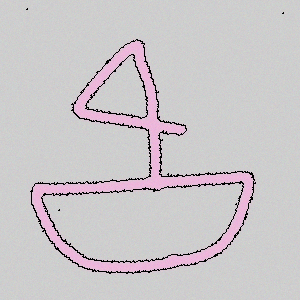
\includegraphics[width=0.25\textwidth]{img/noise_data2_border.png}
	\caption{A thin black border is drawn between clusters.}
	\label{fig:border1}
\end{figure}

Another possible correction procedure is to change the colors or contrast of the image itself. For example. in the sailboat data point in figure \ref{fig:data1}, the pink or the gray could be darkened. This method would leave the picture more intact as it wouldn't draw black lines, which could make the image more cumbersome to look at. However, this color changing would have to be very precise as to not completely alter the image. Changing the boat to black would assuredly make it more visible, but the image is no longer of a pink boat and a gray background. Subtly changing the color values or contrast would ensure that the image is still in tact while being more accessible. With improvements to the system such as user testing this mechanism could be fine tuned to translate an image into a user and color blind friendly picture.


\begin{figure}[H]
	\centering
	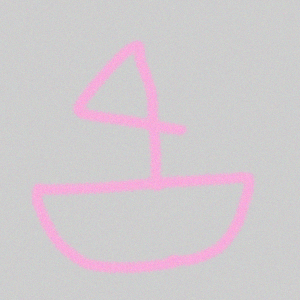
\includegraphics[width=0.25\textwidth]{img/noise_data2_noise_corrected.png}
	\caption{Cluster colors slightly adjusted.}
	\label{fig:corrected1}
\end{figure}


\section{Results Analysis}


The output of this system will be the corrected images. For the scope of this research, wide, comprehensive results will not be provided. Only one person will evaluate whether the objects are easier to distinguish; and indeed they are. Peers were consulted  as to how destructive the algorithm is, that is how much it alters the colors. A proper analysis would involve both groups of color blind and non color blind subjects. They would examine the image before and after processing and comment on the effectiveness and destructiveness. 

\section{Conclusion}
On the whole, this research has outlined the prototype to a system for assisting people with color blindness. Images are ubiquitous on the Internet. This system provides a method for those affected to enjoy and appreciate this information as anyone else could. An ensemble of machine learning mechanisms provide color clustering; these clusters are then used to determine if there will be any potential confusion in the image and corrects accordingly. Importantly, this correction process does not destroy the image, so the message being communicated is not lost to the viewer. The process can be followed in full through the in figure \ref{fig:process}. Further additions have been suggested throughout this paper, but there are yet more that would bring this research to greater heights.

\begin{figure}[H]
	\centering
	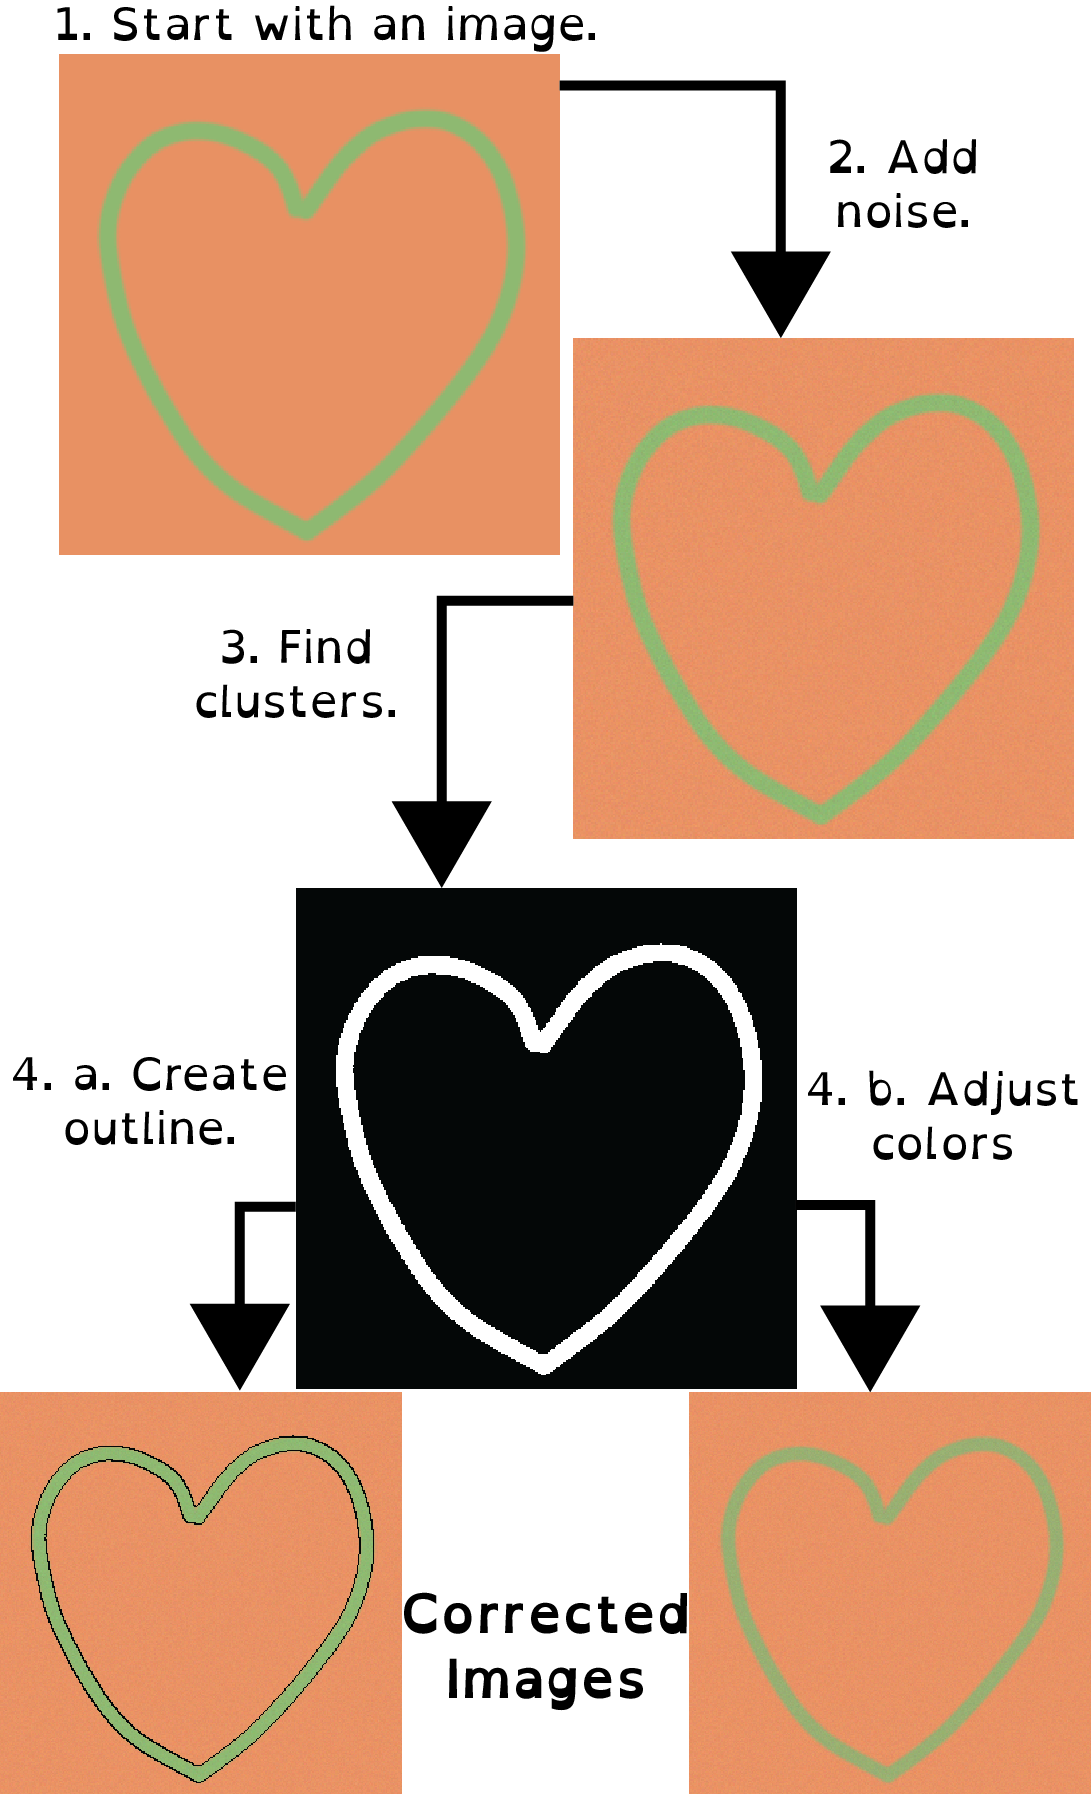
\includegraphics[width=0.7\textwidth]{img/process.png}
	\caption{The correction process.}
	\label{fig:process}
\end{figure}



%\section{To do}
%This project still has a long way to go before it is complete.
%
%\subsection{Color Recognition}
%
%The k-means algorithm seems to be doing a good job clustering the data. I have run it on a few of the sample images that I created and it has successfully segmented the foreground and background properly. I need to further explore other learning tools that can be used here. The current issue:
%
%Finding clusters in a single image is possible. A thin border can be drawn between these sections of the image, adequately distinguishing them to a color blind person. However, how should this be scaled to multiple images? A border need only be drawn between certain pairs of geometrically close colors. That is, if there is pink next to gray (as in the sailboat image) a line would need to be drawn; however, if there is purple in between, such as below, a line probably does not need to be drawn.
%
%\begin{figure}[H]
%	\centering
%	
\includegraphics[width=0.25\textwidth]{img/graypurplepink.png}
%	\caption{Current clustering problems.}
%	\label{fig:kmeans2}
%\end{figure}
% 
%My current plan is to store pixel's cluster as well as its cluster's complement. Thus, if a pixel is found next too a pixel in its complementary cluster, a border can be drawn. 
%
%I plan to achieve this by stacking all of the image data and determining holistic clusters that show up across all of the data rather than examining one image at a time. This will allow for multiple images to share the same clusters and avoid creating two clusters for the same combination. For example, if two images are given containing the colors blue and purple, both blues will be in one cluster and both purples in another.
%
%One potential issue with this approach is miscategorization. For example, if a bunch of red pixels end up in a purple cluster, then the system will essentially be rendered useless.
%
%I also need to further investigate what to do with the clusters after they are found. I do not currently have a way to apply them to other images. I will read more on k-means, but I am thinking of training a supervised neural network to categorize new data once all of the clusters are found. One issue with this yet is that I do not have enough images to train a network. It would be vastly over trained and not adaptable. I will also be investigating principal component analysis.

%\subsection{Color Correction}
%I have not yet determined how I am going achieve non-destructive color correction. I am currently learning towards drawing a border between two complementary clusters. However, I do not know how to find the border between these. I do not yet have the knowledge of graphics required to go through the pixels and compare them efficiently. I do not think this will be too difficult, but I think devising a solution to this problem will take a lot of time. 
%
%My current plan is to go through each pixel, check its cluster and compare that to the clusters of the pixels surrounding it. If a neighbor is found to be in a complementary cluster, then the pixel will be changed to black (i.e. part of the border). Its primary cluster will not be changed so that its neighbors are not necessarily changed. This primitive approach does not seem computationally efficient. It would take width$\times$height$\times 4$ comparisons for each image. The test images that I have created are 300 by 300, which would require 360000 comparisons. I have not researched this area yet, but I hope to find a more efficient algorithm for iterating through my data.

%\section{Progress Report Update}
%
%With advisement from Dr. Deppa from the Statistics department, I have devised a way to reduce over fitting. Currently, the background of my images are a solid color and the foreground are slightly fuzzy around the edges. This will result in a cluster of entirely one color (i.e. the background) and one of mostly one color, but some variety due to the edge fuzz. Training a clustering algorithm on this data will work for a test image, but will not cross validate nor test well. For a pixel to be in the first cluster, it will have to be a very specific color.
%
%To combat this, I am adding normal noise to the colors of my pixels. This will add some variety to each pixel, incurring the fuzziness desired to help reduce the over fitting. 
%
%I am still looking into how I will stack the data. Stacking allows for all the data to be analyzed at once. This would be convenient for an over night training session and to train the clusters all together. Thus, I would have consistent clusters across all of my data. This will allow for a more holistic approach to training my final network. For example, all of my blues will be in the same cluster, rather than in their own clusters by image. However, it will then be harder to find complementary clusters.
%
%One idea that I am playing with is adding an Image ID field to the data. Then the clusters in two images are known to be complementary, but the data can still be stacked. 
%
%I am looking into simple RGB scaling to convert neighboring, conflicting clusters instead of drawing an edge. 
%
%A good final test for the system (Data Analysis) would be to send some legitimate Ishihara samples through the trained network to see if they are properly clustered and dealt with.

\section{Future Improvements}
\subsection{Better Data}
The data is currently created by one person that is red-green color blind. This is a humble start, everyone's color blindness is a little different. Thus, creating data that caters to only one person may leave out issues experienced by many other people with red-green and blue-yellow color deficiencies.

To solve this problem, the National Eye Institute or even an eye doctor could be inquired about the data. They could judge the data set created to see if there are any glaring cases missing from examination. Alternatively, they could provide the data themselves. These expert analysis of the problem would make the system more reliable.

\subsection{Including Users in the Development}
Any good software is going to include some sort of user testing. In this case, the users could help refine both the data and the correction functionality. Similar to an expert's opinion, getting feedback from many users will help create reliable data. This will ensure that no color combinations go un-learned by the system. 

After the system has learned with a more inclusive data set, the users could also help judge the color correction. They could be given before and after pictures; offering their input as to whether the system actually accomplished its goal of helping them distinguish the colors in the image. Additionally, a non-color blind group of people could be brought in, again given the before and after pictures. These participants would be able to determine how drastic a change the system made to the image. Combining feedback from these two groups of people would help reach an equilibrium between making an image more accessible while not altering its meaning.


\pagebreak
\section{References}
\bibliography{bibliography}{}
\bibliographystyle{plain}


\end{document}
